%%%%%%%%%%%%%%%%%% Część I %%%%%%%%%%%%%%%%%

\section{Uczenie nadzorowane warstwowych sieci neuronowych}

\subsection{Różnice funkcjonalne pomiędzy sieciami jedno- i wielowarstwowymi oraz pomiędzy sieciami liniowymi a nieliniowymi (uczenie sieci warstwowych funkcji logicznej AND i funkcji różnicy symetrycznej XOR)}

\begin{enumerate}
\item \textbf{
Skonstruuj zbiór przykładów definiujący dwuargumentową funkcję ("bramkę") AND (File|New|Data set) i zachowaj go. Wszystkie 4 przykłady mają stanowić zbiór uczący. Jakie są klasy decyzyjne w tym zbiorze przykładów i jakie są ich liczności?}

\item \textbf{
Wyszukaj w Pomocy hasło "Verification" i przeczytaj wszystkie pięć znalezionych tematów.}

\item \textbf{
Wyobraź sobie (narysuj) pożądaną funkcję odpowiedzi sieci (trójwymiarowy wykres zależności wyjścia od dwóch wejść).}

\item \textbf{
Skonstruuj liniową sieć jednowarstwową o architekturze 2-1 (File|New|Network, Type=Linear, przycisk Advise). Uaktywnij okno wykresu błędu średniokwadratowego (Statistics|Training graph). Naucz sieć na problemie AND (Train|Multilayer perceptron|Back propagation). Obejrzyj funkcję odpowiedzi sieci (Run|Responce surface) i błędy dla poszczególnych przypadków (Statistics|Case errors).}

\begin{figure}[h]
\centering
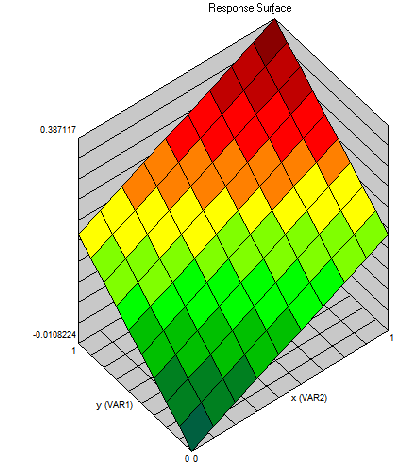
\includegraphics[scale=1.0]{dane/part1/zad2/response}
\caption{Funkcja odpowiedzi sieci.}
\label{fig:response_nonlinear}
\end{figure}

\begin{figure}[h]
\centering
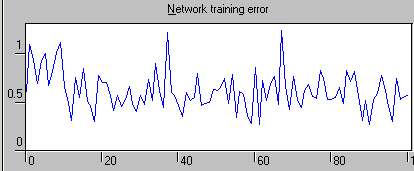
\includegraphics[width=0.6\textwidth]{dane/part1/zad2/error}
\caption{Błąd średniokwadratowy.}
\label{fig:error_nonlinear}
\end{figure}

\begin{figure}[h]
\centering
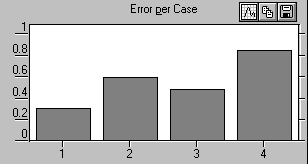
\includegraphics[width=0.6\textwidth]{dane/part1/zad2/error_case}
\caption{Błąd dla poszczególnych przypadków.}
\label{fig:error_nonlinear}
\end{figure}
\paragraph{Jak widać sieć nie radzi sobie z zadaniem - przez swą linoiwą naturę zawsze średnia wartość funkcji w punktach (0,1) i (1,0)  będzie równa średniej wartości w punktach (0,0) i (1,1) przez co wagi mogą jedynie zmienić rozłożenie błędu między poszczególne przypadki uczące, ale zawsze zmniejszanine błędu w punktach (0,0), (0,1) i (1,0) będzie powodowało wzrost błędu w punkcie (1,1) i na odwrót. Przy zmniejszeniu prędkości uczenia błąd sieci można zredukować do ok 0.2.}

\item \textbf{
Spróbuj utworzyć sieć liniową dla problemu AND o liczbie warstw większej niż 2.}
\paragraph{Porgram nie pozwala na utworzenie takiej sieci, ponieważ nie ma to sensu - po dodaniu dodatkowych warstw końcowa funkcja aktywacji będzie tylko kombinacją liniową funkcji poszczególnych neuronów. Dodatkowe warstwy są redundantne, ponieważ dla każdej liniowej sieci 3 i więcej warstwowej istnieje odpowiadająca jej sieć 2 warstwowa, której zachowanie jest identyczne.}
\item \textbf{
Przerób sieć na nieliniową sieć jednowarstwową (ustawiając Act fn w Edit|Network na Logistic) i naucz ją na tym samym problemie.}

\begin{figure}[h]
\centering
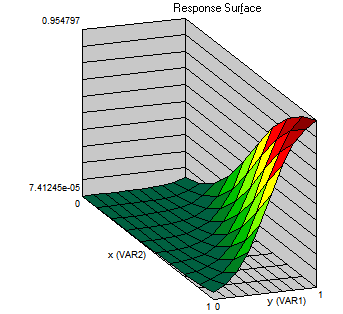
\includegraphics[scale=1.0]{dane/part1/zad2/response_nonlinear}
\caption{Funkcja odpowiedzi sieci.}
\label{fig:response_nonlinear}
\end{figure}

\begin{figure}[h]
\centering
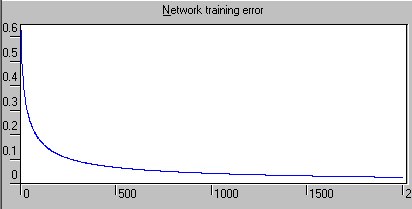
\includegraphics[width=0.6\textwidth]{dane/part1/zad2/error_nonlinear}
\caption{Błąd średniokwadratowy.}
\label{fig:error_nonlinear}
\end{figure}

\begin{figure}[h]
\centering
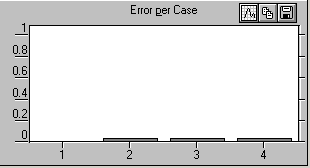
\includegraphics[width=0.6\textwidth]{dane/part1/zad2/error_case_nonlinear}
\caption{Błąd dla poszczególnych przypadków.}
\label{fig:error_nonlinear}
\end{figure}

\paragraph{Sieć nielinowa poradziła sobie z problemem znacznie lepiej - błędy klasyfikacji bliskie zeru. W przeciwieństwie do sieci liniowej widać, że proces uczenia jest zbieżny - wraz z uczeniem błąd asymptotycznie maleje.
}
\item \textbf{
Wejdź do edytora sieci (Network|Edit) i przypatrz się wagom neuronu wyjściowego. Wykreśl w przestrzeni wejść prostą, którą definiuje neuron wyjściowy i oceń, czy i jak realizuje ona separację klas decyzyjnych. }


\begin{figure}[h]
\centering
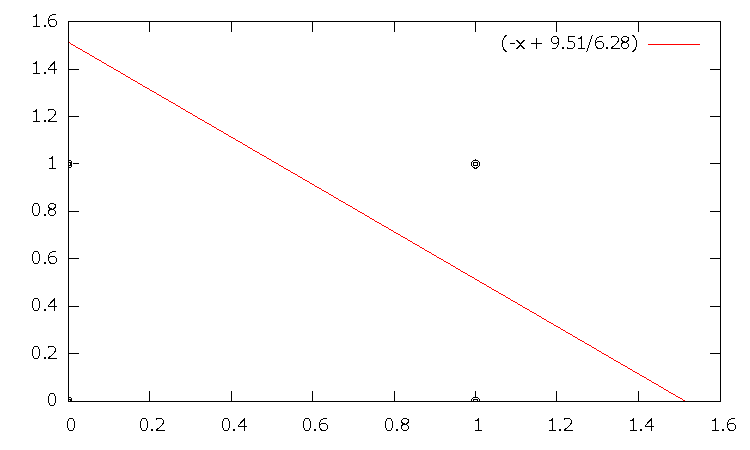
\includegraphics[width=0.8\textwidth]{dane/part1/zad2/oska}
\caption{Prosta separująca klasy decyzyjne.}
\label{fig:prosta_separujaca}
\end{figure}

\paragraph{Prosta dobrze realizuje separację klas decyzyjnych - oddziela 3 przypadki o wartości 0 od przypadku o wartości 1}

\item \textbf{
Skonstruuj zbiór przykładów definiujący dwuargumentową funkcję XOR i zachowaj go. Wszystkie 4 przykłady mają stanowić zbiór uczący.}

\item \textbf{
Wyobraź sobie (narysuj) pożądaną funkcję odpowiedzi sieci.}

\item \textbf{
Skonstruuj liniową sieć jednowarstwową o architekturze 2-1 i naucz ją na problemie XOR.}

\item \textbf{ Obejrzyj funkcję odpowiedzi sieci i błędy dla poszczególnych przypadków.}

\item \textbf{
Przerób sieć na nieliniową sieć jednowarstwową i naucz ją na tym samym problemie (zwróć uwagę, jak sieć stara się minimalizować błąd). Obejrzyj, jak zmienia się rozkład wag podczas procesu uczenia (Statistics|Weight distribution).}

\item \textbf{
Skonstruuj nieliniową sieć dwuwarstwową o architekturze 2-2-1 (File|New|Network, Type=Multilayer perceptron) i naucz ją na problemie XOR. Obejrzyj funkcję odpowiedzi.}

\item \textbf{
Obejrzyj wagi sieci w edytorze sieci (Edit|Network). Jakie proste definiują neurony w warstwie ukrytej (spróbuj je narysować w przestrzeni wejść) ? Jak można interpretować działanie neuronu wyjściowego ?}

\item \textbf{
Obejrzyj, jak zmienia się rozkład wag podczas procesu uczenia. Jaka jest przyczyna takiego zachowania wag i jakie to może mieć konsekwencje (z "informatycznego" punktu widzenia) ?}
\end{enumerate}

\subsection{Obserwacja zjawiska przeuczenia na przykładzie zbioru PIMA.}
\begin{enumerate}
\item \textbf{ Zapoznaj się z pochodzeniem zbiorów PIMA i BUPA (wyszukaj: "PIMA dataset", "BUPA dataset").}

\item \textbf{
Wczytaj zbiór PIMA i skonstruuj dla niego dwuwarstwową sieć nieliniową o architekturze 8-4-1.}

\item \textbf{
Obejrzyj ustawienia w okienku Pre/Post Processing.}

\item \textbf{
Wyłącz "inkrementacyjne" warunki stopu ustawiając np. zero lub dużą wartość parametru Window w oknie Stopping Conditions.}

\item \textbf{
Przeprowadź uczenie algorytmem wstecznej propagacji błędu (może być bardzo długie, np. 20 000 epok); obserwuj przebieg błędu dla zbioru uczącego i weryfikującego.}
\end{enumerate}

\subsection{Dobór liczby neuronów w warstwie ukrytej na przykładzie zbioru IRIS.}
\begin{enumerate}
\item \textbf{ Dla zbioru IRIS przeprowadź co najmniej 5 eksperymentów uczenia nieliniowych sieci dwuwarstwowych o architekturach 4-n-3, dla n zmieniającego się w przedziale [2,10], przy wyłączonym kryterium warunku stopu na zbiorze weryfikacyjnym. Po każdym eksperymencie kopiuj przebieg błędu przez schowek do Notatnika.}

\item \textbf{
Przedstaw w gnuplocie na jednym wykresie przebieg błędu uczenia dla kolejnych wartości n.}

\item \textbf{
Czy istnieje jednoznaczna zależność pomiędzy n a przebiegiem błędu średniokwadratowego? Czy biorąc pod uwagę tylko przebeg błędu dla zbioru uczącego można ustalić optymalną liczbę neuronów w warstwie ukrytej? Jeśli tak, to ile ona wynosi dla tego zbioru przykładów?}
\end{enumerate}

\subsection{Sterowanie rozmiarem obszaru niepewnych odpowiedzi (braku odpowiedzi) sieci na granicach klas decyzyjnych (podczas testowania sieci)}
\begin{enumerate}
\item \textbf{Utwórz i naucz sieć na zbiorze PIMA (architektura 8-4-1).}

\item \textbf{
Przeprowadź klasyfikowanie przykładów ze zbioru testującego (okno Statistics|Classification). Znajdź w tym oknie macierz pomyłek (ang. confusion matrix).}

\item \textbf{
Otwórz okno Edit|Pre-Post Processing. Pola Accept i Reject definiują, jakie wartości muszą mieć neurony w warstwie wyjściowej, aby móc zinterpretować ich stan jako decyzję o przypisaniu przykładu do odpowiedniej klasy decyzyjnej. Choć nie jest to kontrolowane przez program, powinno zachodzić Accept >= Reject}

\item \textbf{
Przy użyciu gnuplota sporządź wykres (trzy przebiegi na jednym wykresie) zależności procentu przypadków z jednego ze zbiorów (uczącego / weryfikującego / testującego):
– poprawnie zaklasyfikowanych (do wszystkich klas decyzyjnych razem),
– niepoprawnie zaklasyfikowanych,
– niezaklasyfikowanych
w funkcji progu Accept, dla następujących wartości Accept i Reject:
\begin{tabular}{|c|c|}
\hline Accept & Reject \\ 
\hline 0.5 & 0.5 \\ 
\hline 0.6 & 0.4 \\ 
\hline 0.7 & 0.3 \\ 
\hline 0.8 & 0.2 \\ 
\hline 0.9 & 0.1 \\ 
\hline 1.0 & 0.0 \\ 
\hline 
\end{tabular} 
}

\item \textbf{
Czy na podstawie otrzymanego wykresu można zasugerować jakąś optymalną wartość obu progów dla tego zbioru przykładów i tej sieci?}

\end{enumerate}

\subsection{Badanie odporności sieci na uszkodzenia}
\begin{enumerate}
\item \textbf{Skonstruuj sieć dwuwarstwową o architekturze 4-3-3 dla problemu IRIS i naucz ją.}

\item \textbf{
Przeprowadź testowanie i zapisz trafność klasyfikowania.}

\item \textbf{
Otwórz edytor sieci (Edit|Network). Wyszukaj (w obu warstwach: ukrytej i wyjściowej!) i usuń z sieci (tj. wyzeruj) wagę najmniejszą co do wartości bezwzględnej (pomiń wiersz Threshold, zawierający progi neuronów). Przeprowadź ponownie testowanie sieci i zapisz wynik.}

\item \textbf{
Kroki z punku 3 powtórz ok. 10 razy, kolejno usuwając coraz większe wagi i notując trafność klasyfikowania. Sporządź wykres zależności trafności klasyfikowania w funkcji ilości usuniętych (najmniejszych) wag.}

\item \textbf{
Czy odporność sieci na uszkodzenia (usunięcia wag) jest wysoka?}

\item \textbf{
Czy jesteś w stanie na podstawie tak “zredukowanej” sieci powiedzieć coś o ważności poszczególnych atrybutów opisujących przykłady?}

\item \textbf{
Czy w konsekwencji “przerzedzenia” sieci można usunąć niektóre neurony? Jak należy to zrobić? (przemyśl dokładnie).}
\end{enumerate}

\subsection{ Eksperymentalny dobór rozmiaru zbioru weryfikującego}
\paragraph{Dla zbioru IRIS, PIMA lub BUPA przeprowadź eksperyment uczenia i testowania, zmieniając proporcje pomiędzy zbiorem uczącym i weryfikującym.}
\begin{enumerate}
\item \textbf{Zacznij od następujących proporcji zbioru uczącego, weryfikującego i testującego 8:1:1.}

\item \textbf{
Przeprowadź uczenie (liczba epok >=300). Przetestuj sieć, zapisz trafność klasyfikowania, błąd klasyfikowania i procent przykładów niezaklasyfikowanych.}

\item \textbf{
Sukcesywnie zwiększaj rozmiar zbioru weryfikującego, zmniejszając rozmiar uczącego (pole Training w oknie Edit|Data set), do proporcji 1:8:1 włącznie.}

\item \textbf{
Sporządź wykres zależności trafności klasyfikowania, błędu klasyfikowania i procentu przykładów niezaklasyfikowanych w funkcji proporcji rozmiaru zbioru weryfikującego do liczby przykładów, jakie mamy do dyspozycji podczas uczenia (czyli rozmiar zbioru uczącego + rozmiar zbioru weryfikującego). Czy można znaleźć jakąś wielkość optymalną?
}
\end{enumerate}

\subsection{Porównanie ‘vanilla’ backpropagation z bardziej wyrafinowanymi algorytmami uczenia nadzorowanego sieci warstwowych}
\paragraph{Dla zbioru PIMA lub BUPA przeprowadź eksperyment uczenia i testowania, używając poza standardowym (vanilla) algorytmem backpropagation innych algorytmów uczenia (np. QuickPropagation, Delta-bar-Delta). Dla zapewnienia porównywalności wyników, w poszczególnych eksperymentach zachowaj tą samą konfigurację sieci i warunki stopu. W miarę możliwości uśrednij wyniki z kilku przebiegów dla każdego algorytmu. Czy któryś z algorytmów jest wyraźnie lepszy? Porównaj liczbę epok uczenia.}
\paragraph{
Uwaga. Algorytmy QuickProp i DeltaBarDelta mogą okazać się trochę niestabilne (w ogólności łatwiej niż backprop wpadają w minima lokalne). W takim przypadku trzeba się trochę pobawić parametrami.}

\subsection{Inne sieci warstwowe – sieci z jednostkami o symetrii kołowej (RBF)}
\begin{enumerate}
\item \textbf{Zbuduj sieć RBF dla problemu IRIS.
Otwórz edytor sieci (Edit|Network). Zwróć uwagę na różnice w polach Act fn i PSP in w porównaniu z perceptronami.}

\item \textbf{
Naucz sieć. Uczenie składa się z trzech etapów: ustalania centrów poszczególnych neuronów, ustalenia promieni (deviation), które decydują o stopniu “spłaszczenia” funkcji Gaussowskich, oraz obliczenia wag neuronu wyjściowego. Zwróć uwagę na czas uczenia.}

\item \textbf{
Obejrzyj funkcję odpowiedzi wybranych neuronów w warstwie ukrytej i neuronów w warstwie wyjściowej (Run|Response Surface). Możesz zmieniać też zmienne niezależne (atrybuty). Zauważ różnice w stosunku do sieci z jednostkami logistycznymi.}

\item \textbf{
Zastanów się, jakie konsekwencje ma niewłaściwy dobór promieni. Co będzie się działo, gdy promienie będą za duże? Co, gdy za małe? (związek z generalizacją).}

\item \textbf{
Przetestuj sieć dla różnych metod uczenia, tj. dla różnych inicjalizacji centrów (Sample, K-means) i różnych sposobów ustalania odchyleń (Explicit, Isotropic, K-nearest). Najlepiej miej otwarty edytor sieci; obserwuj jakie konsekwencje ma wybranie poszczególnych sposobów uczenia.}

\item \textbf{
Porównaj sieć RBF z siecią typu Multilayer Perceptron na trudniejszym zbiorze przykładów (PIMA lub BUPA).}
\end{enumerate}

\subsection{ Uzyskiwanie jak najwyższej trafności}
\paragraph{Manipulując:}
\begin{itemize}
\item \textbf{architekturą sieci,}
\item \textbf{prędkością uczenia (można zmieniać dynamicznie),}
\item \textbf{zakresem wartości używanych do inicjalizacji wag sieci,}
\item \textbf{warunkami stopu (statycznymi i/lub dynamicznymi),}
\item \textbf{rodzajem algorytmów,}
\end{itemize}
\paragraph{spróbuj uzyskać jak największą trafność klasyfikowania na zbiorze testującym dla zbioru PIMA lub BUPA.
\\Jeśli możesz, porównaj uzyskany wynik z trafnością otrzymaną przy użyciu drzew decyzyjnych.
\\Aby zapewnić porównywalność wyników i powtarzalność eksperymentu, nie zmieniaj oryginalnego przyporządkowania przykładów do zbiorów uczącego, weryfikującego i testującego.}